\documentclass[conference]{IEEEtran}

% ---------- Robust UTF-8 & fonts (pdflatex / xelatex 両対応) ----------
\usepackage{iftex}
\ifPDFTeX
  \usepackage[utf8]{inputenc}
  \usepackage[T1]{fontenc}
  \usepackage{lmodern}
\else
  \usepackage{fontspec} % xelatex/lualatex
\fi

% ---------- Common packages ----------
\usepackage{graphicx}
\usepackage{amsmath}
\usepackage{cite}
\usepackage{url}
\usepackage[hidelinks]{hyperref}
\usepackage{booktabs}
\usepackage{tikz}
\usepackage{pgfplots}
\pgfplotsset{compat=1.18}

\begin{document}

\title{Pb-free ScAlN MEMS Array Integrated with 65 nm SiGe CMOS via System-in-Package for Medical Ultrasonic Sensors}

\author{
  \IEEEauthorblockN{Shinichi Samizo}
  \IEEEauthorblockA{Independent Semiconductor Researcher\\
  Former Engineer at Seiko Epson Corporation\\
  Email: \href{mailto:shin3t72@gmail.com}{shin3t72@gmail.com}\\
  GitHub: \url{https://github.com/Samizo-AITL}}
}

\maketitle

\begin{abstract}
Conventional medical ultrasonic devices have been dominated by PZT (Pb(Zr,Ti)O$_3$)~\cite{akata2009pzt}. However, Pb-containing materials face strict regulatory restrictions (EU RoHS, REACH, FDA) in in-body medical applications. This work proposes a Pb-free alternative based on ScAlN MEMS arrays, integrated with 65~nm SiGe CMOS using System-in-Package (SiP) technology.
The ScAlN MEMS array is designed for 10--50~MHz operation with $\lambda/2$ pitch for high-resolution imaging~\cite{akrout2018scaln}. The SiGe CMOS front-end integrates LNA, VGA, and ADC, enabling detection of microvolt-level signals. The SiP approach ensures yield separation, short interconnects, and hermetic sealing for medical reliability. Finite element and circuit simulations indicate adequate sensitivity and beam directivity at 20--40~MHz, LNA noise figure $<2$~dB, and compact, reliable packaging via flip-chip SiP. Pb-free ScAlN arrays with 65~nm SiGe CMOS via SiP form a practical path for next-generation high-resolution medical ultrasonic sensors.
\end{abstract}

\begin{IEEEkeywords}
ScAlN MEMS, Pb-free piezoelectrics, System-in-Package (SiP), SiGe CMOS, Medical ultrasound, Ultrasonic imaging
\end{IEEEkeywords}

\section{Introduction}
Medical ultrasonic imaging is widely used in ophthalmology, vascular diagnosis, dermatology, and implantable monitoring. Traditional devices have been dominated by PZT due to superior piezoelectric properties~\cite{akata2009pzt}, but Pb toxicity limits in-body use under EU RoHS, REACH, and FDA regulations. Scandium-doped AlN (ScAlN) has emerged as a Pb-free candidate with CMOS compatibility, high-$Q$, and industrial adoption in RF BAW/XBAR filters~\cite{akrout2018scaln}. We propose ScAlN MEMS arrays co-integrated with 65~nm SiGe CMOS via SiP for medical ultrasound.

\section{Background and Contributions}
\subsection{Background}
PZT transducers provide excellent $d_{33}$ and coupling but contain Pb and are not preferred for in-body devices~\cite{akata2009pzt}. CMUT/PMUT enable MEMS-CMOS co-integration, yet often require high bias and face fluid-reliability challenges~\cite{khuri2009cmut}. ScAlN is a promising Pb-free piezoelectric with proven manufacturability and CMOS process compatibility~\cite{akrout2018scaln}. Combining ScAlN arrays with low-noise SiGe readout via SiP offers a realistic, compliant route to high-resolution ultrasound.

\subsection{Contributions}
\begin{itemize}
  \item Pb-free ScAlN MEMS array architecture for 10--50~MHz imaging.
  \item Heterogeneous integration with 65~nm SiGe CMOS via SiP to minimize interconnect and improve SNR.
  \item FEM/circuit examples indicating adequate sensitivity, beam directivity, and low-noise detection at 20--40~MHz.
  \item Application considerations in ophthalmology~\cite{pavlin2009ubm}, IVUS~\cite{foster2000ivus}, dermatology, and implantables.
\end{itemize}

\section{System Concept}
\subsection{ScAlN MEMS Array}
Operation: 10--50~MHz. Channels: 64--256 with $\lambda/2$ pitch. Structures: PMUT-like stacks or BAW/XBAR cavities.

\subsection{SiGe CMOS Front-end}
65~nm SiGe BiCMOS with low NF ($<2$~dB). Integrated LNA, VGA, ADC, and T/R switch to sense $\mu$V-level signals.

\subsection{System-in-Package Integration}
Flip-chip bonding integrates MEMS and CMOS dice. Benefits: yield separation, short interconnects, and hermetic sealing.

\begin{figure}[t]
\centering
\begin{tikzpicture}[node distance=1.6cm, auto, thick]
\tikzstyle{blk}=[rectangle,draw,rounded corners,minimum height=9mm,minimum width=26mm,align=center]
\node[blk] (mems) {ScAlN MEMS Array\\(10--50 MHz)};
\node[blk, right=12mm of mems] (lna) {SiGe LNA/VGA\\(65 nm)};
\node[blk, right=12mm of lna] (adc) {ADC\\(12--14 bit, 50--100 MS/s)};
\node[blk, right=12mm of adc] (bf) {Beamformer/\\Digital Core};
\draw[->] (mems)--(lna);
\draw[->] (lna)--(adc);
\draw[->] (adc)--(bf);
\end{tikzpicture}
\caption{System architecture (ScAlN MEMS + 65~nm SiGe via SiP).}
\label{fig:arch}
\end{figure}

\section{Simulation Results}
FEM analysis confirms resonances at 20, 30, and 40~MHz with $k^2_{\mathrm{eff}}\!=\!2$--4\%. Circuit estimates show LNA input noise $<2$~nV/$\sqrt{\mathrm{Hz}}$ and system SNR $>60$~dB at 20--40~MHz.

\begin{figure}[t]
\centering
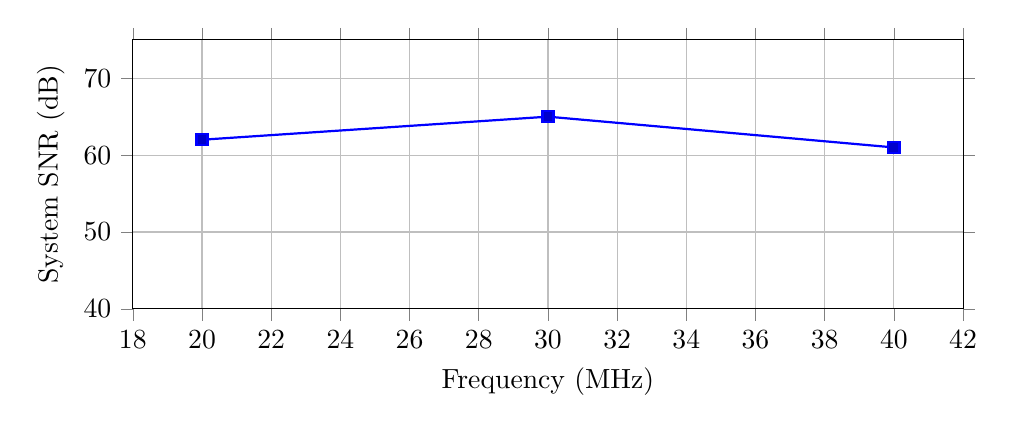
\begin{tikzpicture}
\begin{axis}[
  width=\columnwidth,height=5.0cm,
  xlabel={Frequency (MHz)}, ylabel={System SNR (dB)},
  xmin=18,xmax=42,ymin=40,ymax=75, grid=both, tick align=outside]
\addplot+[mark=square*,thick] coordinates {(20,62) (30,65) (40,61)};
\end{axis}
\end{tikzpicture}
\caption{Example system SNR with SiGe front-end.}
\label{fig:snr}
\end{figure}

\begin{table}[t]
\caption{System Specifications (ScAlN Array + 65 nm SiGe via SiP)}
\label{tab:spec}
\centering
\begin{tabular}{@{}ll@{}}
\toprule
\textbf{Parameter} & \textbf{Specification}\\
\midrule
Operating frequency & 10--50 MHz\\
Array size & 64--256 ch (1D/2D)\\
Pitch rule & $\lambda/2$ (tissue $c\!\approx\!1540$ m/s)\\
CMOS node & 65 nm SiGe BiCMOS\\
Front-end blocks & LNA, VGA, T/R switch, ADC\\
ADC resolution & 12--14 bit, 50--100 MS/s\\
System SNR & $>60$ dB (20--40 MHz)\\
Package & SiP (flip-chip)\\
\bottomrule
\end{tabular}
\end{table}

\begin{table}[t]
\caption{Piezoelectric Materials for Ultrasonic MEMS (Summary)}
\label{tab:mat}
\centering
\begin{tabular}{@{}lllll@{}}
\toprule
Material & Pb-free & $d_{33}$ & CMOS & Notes\\
\midrule
PZT  & No  & 100--500 & Low  & High performance\\
ScAlN& Yes & 20--30   & High & CMOS-compatible\\
KNN  & Yes & 80--200  & Med. & Bulk ceramic\\
BNT  & Yes & $\sim$100& Med. & High-temp stable\\
ZnO  & Yes & 10--15   & High & Simple, low $d_{33}$\\
PVDF & Yes & 5--10    & High & Flexible, low output\\
\bottomrule
\end{tabular}
\end{table}

\section{Application Scenarios}
\begin{itemize}
  \item \textbf{Ophthalmology:} 20--40~MHz anterior eye imaging~\cite{pavlin2009ubm}.
  \item \textbf{Vascular IVUS:} 30--40~MHz catheter arrays~\cite{foster2000ivus}.
  \item \textbf{Dermatology:} 10--20~MHz skin/tumor imaging.
  \item \textbf{Implantables:} Miniaturized SiP with telemetry.
\end{itemize}

\section{Discussion}
Versus PZT, ScAlN offers CMOS compatibility and Pb-free compliance at lower $d_{33}$. Versus CMUT/PMUT~\cite{khuri2009cmut}, ScAlN needs lower bias and shows better fluid reliability. SiP yields separation, short interconnects, and hermeticity versus monolithic integration.

\section{Conclusion}
Pb-free ScAlN MEMS arrays integrated with 65~nm SiGe CMOS via SiP provide: (i) regulatory compliance, (ii) adequate 20--50~MHz resolution, (iii) low-noise detection via SiGe, and (iv) scalable, reliable packaging. This is a practical, competitive path for next-generation medical ultrasonic sensors.

\section*{Acknowledgment}
The author thanks colleagues and collaborators in semiconductor device research and MEMS development.

\bibliographystyle{IEEEtran}
\bibliography{references}

\section*{Author Biography}
\textbf{Shinichi Samizo} received the M.S. degree in Electrical and Electronic Engineering from Shinshu University, Japan. He joined Seiko Epson Corporation in 1997, engaging in semiconductor device process development including 0.25--0.18~$\mu$m CMOS, HV-CMOS, DRAM, FeRAM, and FinFET/GAA research. He also contributed to inkjet MEMS process development and thin-film piezo actuator design, leading to the productization of PrecisionCore printheads. His expertise covers semiconductor devices (logic, memory [DRAM/FeRAM/SRAM], high-voltage mixed integration), inkjet actuators, and AI-based control education.

\end{document}
